\documentclass{book}

%\usepackage[norsk]{babel}
\usepackage{times,amssymb,amsmath}
\usepackage[dvips]{epsfig}
\usepackage{natbib}
\usepackage{a4wide}
\usepackage{t1enc}
\newcommand{\matpiv}{{\bf MatPIV~}}
\title{An introduction to {\bf MatPIV} v. 1.6.1}
\author{Johan Kristian Sveen\\
{\small Center for Mathematical Sciences,} \\
{\small Department of Applied Mathematics and Theoretical Physics,} \\
{\small University of Cambridge, UK}}

\date{\today}
\begin{document}

\maketitle


\chapter*{License}

This program is free software; you can redistribute it and/or modify it
under the terms of the GNU General Public License as published by the
Free Software Foundation; either version 2 of the License, or (at your
option) any later version. This program is distributed in the hope that
it will be useful, but WITHOUT ANY WARRANTY; without even the implied
warranty of MERCHANTABILITY or FITNESS FOR A PARTICULAR PURPOSE. See the
GNU General Public License for more details.

The GNU General Public License can be found on the World Wide Web at
http://www.gnu.org/copyleft/gpl.html or it can be obtained by writing to
the Free Software Foundation, Inc., 59 Temple Place - Suite 330, Boston,
MA 02111-1307, USA.




\tableofcontents
\newpage
\chapter*{Introduction}

MatPIV is a program written for the authors personal educational
purposes only and should be treated thereafter. This document acts
primarily as an entry level documentation to the MatPIV m-files and the
Particle Image Velocimetry method used here. Users/Readers are advised
to consult my review paper on PIV~\citep{Sveen:2004}, a decent book on the
subject, e.g.~\cite{Raffel:1998}, the PhD thesis
by~\cite{Westerweel:1993}, and finally the various articles written by
different authors over the last decade or so (some references are
included in the bibliography list). 

The \matpiv distribution comes with 3 different sets of demo-images
which are taken from the papers by~\cite{Grue:1999}
and~\cite{Jensen:1999}.

The \matpiv files have been tested on Linux machines only, with MATLAB
versions from 5.2.1.1420 and up to 6.5.0. It is recommended that users
have the Image processing toolbox, although a few workarounds do
exist.

The aim of the present document is primarily to give an overview of the
functionality of the \matpiv toolbox. At the time of writing, \matpiv is
one of at least three available, free toolboxes. It is, however, by far
the largest presently available, both when functionality and number of
users are considered. Interested readers may google for {\bf UraPIV} and
{\bf mpiv} to find alternative PIV-software.

\chapter{Installation}

\matpiv is distributed as zipped archives which may be downloaded from
the \matpiv webpage. 

\section{Unix/Linux}
This comes in the form of a single tar.gz file which should be installed
in the following steps: 1) create a directory called, say, MatPIV1.6.1
and cd to it. 2) type
\begin{verbatim}
~> tar -zxvf MatPIV1.6.1.tar.gz 
\end{verbatim}

\section{Windows}
This comes in the form of a zip-archive. Install by first creating a
directory called, say, MatPIV1.6.1 and then unzipping the archive into
it (using your preferred zip-utility).

\section{Adding the path to Matlab}
Subsequently you need to add this directory and all it's subdirectories
to the {\bf Matlab} path. This can be done in a few different ways.
Firstly, if you are running {\bf Matlab} with it's full desktop, you can
click 'File', 'Set Path', followed by 'Add with sub-folders' and finally
adding your newly created directory.

Alternatively for Unix/Linux users, you can add a file named {\em
startup.m} to your home-directory, containing the following lines
\begin{verbatim}
p=genpath('/the/path/where/you/installed/MatPIV1.6.1');
addpath(p);
\end{verbatim}
This assumes you always start up {\bf Matlab} from the root of your
home-directory. If not, the paths are not added.


\chapter{An example session}
In this section we will take a look at an example session with {\bf
MatPIV}. The images can be found in the ``Demo3''-subdirectory of your
\matpiv{}-installation, and they are taken from an experiment concerning
surface waves in water~(\cite{Jensen:1999}). The images are shown in
figure~\ref{fig:mpimages}.

\section{The easy way}
We can quite easily perform our first PIV-calculation by changing to the
{\em Demo3} directory and executing the command
\begin{verbatim}
>> [x,y,u,v]=matpiv('mpim1b.bmp','mpim1c.bmp',64,0.0012,0.5,'single');
\end{verbatim}
This will interrogate the images in a single pass using $64\times64$
pixels large interrogation windows with $50\%$ overlap. The term
``single pass'' refers to the fact that the calculation is performed by
looping over the images with only one iteration. It is normally better
to use more iterations and achieve higher accuracy, but we shall return
to these subjects at a later stage.

The result consists of four matrices {\em x, y, u} and {\em v} which
are measured in pixels and pixels/second. The result can be visualized
by issuing the following command:
\begin{verbatim}
>> quiver(x,y,u,v)
\end{verbatim}

This is all well, but normally we prefer to know velocities and
positions in engineering units such as centimeters and seconds. To do
this we need to know how large each pixel in our image is, measured in
physical coordinates. Furthermore, it may in some cases be nice to mask
out particular regions of the flow, in order to save computational time.
For example, there is no need to perform our calculations in the airy
part above the wave-crest in figure~\ref{fig:mpimages}.

\section{The not so easy way}
We will now go through the complete process of measuring the velocities
from the accompanying demo-images. The process is in our case started by
first defining a coordinate system so that we know how far the particles
move, measured in physical coordinates (centimeters or meters) instead
of only ``camera'' coordinates (pixels). Thereafter we apply a mask to
the images to avoid performing calculations where there are no particles
(outside the flow field). Subsequently the images will be interrogated
using a window-shifting technique~\cite[]{Westerweel:1997}. After the
velocity field has been found, a series of filters are applied before
finally all the identified outliers are interpolated using a nearest
neighbor interpolation.

\begin{figure}
%\begin{center}
\makebox{
\setlength{\unitlength}{1mm}
\begin{picture}(120,70)(0,0)
\put(3,5){\epsfig{figure=mpim1b.ps, width=6cm}}
\put(65,5){\epsfig{figure=mpim1b.ps, width=6cm}}
\end{picture}}
\caption[\ ]{\label{fig:mpimages} Surface wave. Field-of-view (FOV) is roughly $30*30$ cm}
\end{figure}

\subsection{Specifying the coordinate system}
In this tutorial we will focus on the practical aspects of PIV and
it's application to real experiments. Our first step to quantify the
velocity fields from the images is to determine how large each pixel
is in the images. We can do this by inserting a grid with points into
the field of view and take an image of it with our camera. Such an
image is shown in figure~\ref{fig:mpwoco}, which shows 10 points that
are $5$cm apart. We can now use the function {\it definewoco.m} to
calculate how large a pixel is in the image and the orientation of our
coordinate system.
\begin{figure}
%\begin{center}
\makebox{
\setlength{\unitlength}{1mm}
\begin{picture}(100,100)(0,0)
\put(15,5){\epsfig{figure=mpwoco_new.ps,height=8cm}}
\end{picture}}
\caption[\ ]{\label{fig:mpwoco} Image of coordinate system.}
\end{figure}
In this example we will use the 6 ``dots'' in the image to define our
coordinate system. In this specific case, the dots are rather large and
have a flat peak. Therefore we will use a special option in {\it
definewoco} that cross-correlates the image with a gaussian bell to
emphasize the center of the peaks. The peaks in question are about 8
pixels in diameter, so we'll pass this information to definewoco.
\begin{verbatim}
>> definewoco('mpwoco.bmp','.');
Please give the approximate width of your points (in pixels -
default is 20). Type 0 here to get old behaviour of definewoco: 8
....calculating....this may take a few seconds.
...Done!
Now mark the crosses you whish to use as coordinate points
Please mark your world coordinate points with left mouse button.
Press ENTER when finished!
Now you need to give the physical coordinates to each of the points specified!
-----------------------
Please enter the world coordinates for the white 
 circle  marked in the current figure (in square parenthesis): [-10 10]
Please enter the world coordinates for the white 
 circle  marked in the current figure (in square parenthesis): [-10 5] 
Please enter the world coordinates for the white 
 circle  marked in the current figure (in square parenthesis): [0 10]  
Please enter the world coordinates for the white 
 circle  marked in the current figure (in square parenthesis): [0 5]   
Please enter the world coordinates for the white 
 circle  marked in the current figure (in square parenthesis): [10 5]
Please enter the world coordinates for the white 
 circle  marked in the current figure (in square parenthesis): [10 10]
Mapping function. (N)onlinear or (L)inear (N/n/L/l): l
Error (norm) = 0.019268
Save coordinate file....specify number >> 
Coordinate mapping factors saved to file:  worldco
\end{verbatim}



In another set of images (Demo 1) included with {\bf MatPIV} (where the
coordinate image file is called {\it woco.bmp}) the peaks are well
defined and we would use the more standard approach
\begin{verbatim}
>> definewoco('woco.bmp','o');
\end{verbatim}

\subsection{Masking out regions of the flow}
We observe that there is an area above the water surface where there
are no particles. In this region we do not want to perform our PIV
calculations and hence we can use the file {\it mask.m}\footnote{The
file {\it mask.m} uses a function from the Image Processing Toolbox by
the Mathworks Inc. For those that do not possess this toolbox there
exists a workaround version called {\it mask2.m}} to mask out this
region of the flow. The file displays the image and the mask is
defined by clicking with the left mouse button, and defining the final
point using the middle mouse button. Figure~\ref{fig:maskim}

\begin{verbatim}
>> mask('mpim1b.bmp','worldco.mat');
Mark your polygon points with the left mouse button.
Press the middle button when you are finished, press
<BACKSPACE> or <DELETE> to remove the previously selected vertex.
Do you whish to add another field to mask? (1 = yes, 0 = no) >> 0
* Calculating the pixel to world transformation using linear mapping - DONE
\end{verbatim}
\begin{figure}
%\begin{center}
\makebox{
\setlength{\unitlength}{1mm}
\begin{picture}(100,100)(0,0)
\put(15,5){\epsfig{figure=maskim.eps,height=8cm}}
\end{picture}}
\caption[\ ]{\label{fig:maskim} Masked image. Red region will be
excluded in the subsequent calculations.}
\end{figure}

\subsection{Calculating velocities}
Now we would like to calculate the velocities from the images. We use
the window shifting technique mentioned above and start off with
$64\times64$ large images and end with $16\times16$ after 6 iterations.
The images are taken with a time separation of $0.0012$s and we will use
$50\%$ overlap of the interrogation regions.

\begin{verbatim}
>> [x,y,u,v,snr,pkh]=matpiv('mpim1b.bmp','mpim1c.bmp',...
[64 64;64 64;32 32;32 32;16 16;16 16],...
0.0012,0.5,'multin','worldco.mat','polymask.mat');  

* Pass No: 1
 No. of vectors: 1094 , Seconds taken: 19.606562.
 Global filter running - with limit: 3 *std [U V] ..... 2 vectors changed
 Local median filter running: ...........................
............2 vectors changed.
 Interpolating outliers: ....4 Nan's interpolated.
   Expanding velocity-field for next pass
 Interpolating outliers: .1 Nan's interpolated.
* Pass No: 2
 No. of vectors: 1094 , Seconds taken: 20.628889.
 Global filter running - with limit: 3 *std [U V] ..... 0 vectors changed
 Local median filter running: ...........................
............3 vectors changed.
 Interpolating outliers: ...3 Nan's interpolated.
   Expanding velocity-field for next pass
 Interpolating outliers: ................218 Nan's interpolated.
* Pass No: 3
 No. of vectors: 4402 , Seconds taken: 17.721477.
 Global filter running - with limit: 3 *std [U V] ..... 1 vectors changed
 Local median filter running: ...........................
...............................................
.....3 vectors changed.
 Interpolating outliers: ....4 Nan's interpolated.
   Expanding velocity-field for next pass
 Interpolating outliers: .1 Nan's interpolated.
* Pass No: 4
 No. of vectors: 4402 , Seconds taken: 17.555643.
 Global filter running - with limit: 3 *std [U V] ..... 0 vectors changed
 Local median filter running: ...........................
...............................................
.....1 vectors changed.
 Interpolating outliers: .1 Nan's interpolated.
   Expanding velocity-field for next pass
 Interpolating outliers: ...............................460 Nan's interpolated.
* Pass No: 5
 No. of vectors: 17673 , Seconds taken: 26.574317.
 Global filter running - with limit: 3 *std [U V] ..... 24 vectors changed
 Local median filter running: ............................
..............................................
..........................................................
...........................257 vectors changed
.
 Interpolating outliers: .................................
................281 Nan's interpolated.
* Final Pass
 - Using 16*16 interrogation windows! 
 No. of vectors: 17673, Seconds taken: 33.649626 
* Calculating the pixel to world transformation using linear mapping - DONE

\end{verbatim}

\subsection{Filtering the result}

The next step is to filter the velocity-fields to remove so called
spurious vectors. These are vectors that occur primarily due to low
image quality in some parts of the image(s). We may, for example, have
regions with insufficient seeding (not enough particles to create a good
pattern for matching), or too many particles so that the image is
saturated locally. Most users should find that applying some or all the
following should work well. In the final step we replace the missing
vector values using a nearest neighbor interpolation.

\begin{verbatim}
>> [su,sv]=snrfilt(x,y,u,v,snr,1.3);
 SnR filter running with threshold value = 1.3  - finished... 
391 outliers identified

>> [pu,pv]=peakfilt(x,y,su,sv,pkh,0.5);
 Peak height filter running ....... 
329 vectors changed 

>> [gu,gv]=globfilt(x,y,pu,pv,3);
 Global filter running - with limit: 3 *std [U V] ..... 
1 vectors changed

>> [mu,mv]=localfilt(x,y,gu,gv,2,'median',3,'polymask.mat');
 Local median filter running: ..............................
............................................................
............................................................
.........1464 vectors changed.

>> [fu,fv]=naninterp(mu,mv,'linear','polymask.mat',x,y);
 Interpolating outliers: ....................................
....................2161 Nan's interpolated.
\end{verbatim}

\subsection{Visualizing the results}
Figure~\ref{fig:velo} shows $1/4$ of the velocity-vectors plotted using
the {\bf Matlab} command {\em quiver}. In this case only every fourth
vector is shown due to the high number of vectors present. The figure
was created with the following commands:
\begin{verbatim}
>> quiver(x(1:4:end),y(1:4:end),fu(1:4:end),fv(1:4:end),2); axis tight
\end{verbatim}

\begin{figure}
\begin{center} 
{\psfig{file=velofield.ps ,width=6cm}}
\end{center}
\caption{Filtered and interpolated velocity-field.}\label{fig:velo}
\end{figure}

It is also possible to use the function {\em magnitude.m} to calculate
the magnitude of each velocity vector,
$(\mbox{fu}^2+\mbox{fv}^2)^{1/2}$. Figure~\ref{fig:magn} was created
using the following commands:
\begin{verbatim}
>> w=magnitude(x,y,fu,fv);
>> pcolor(x,y,w), shading flat, colorbar
\end{verbatim}

\begin{figure}
\begin{center} 
{\psfig{file=magnitude.ps ,width=6cm}}
\end{center}
\caption{Magnitude of velocity.}\label{fig:magn}
\end{figure}

The function {\em vorticity} can be used to calculate vorticity
through 4 different numerical schemes. The following commands were
used to create figure~\ref{fig:vort}:

\begin{verbatim}
>> w=vorticity(x,y,fu,fv,'circulation');
>> pcolor(x(2:end-1,2:end-1),y(2:end-1,2:end-1),w), shading flat, colorbar
\end{verbatim}

\begin{figure}
\begin{center} 
{\psfig{file=vorticity.ps ,width=6cm}}
\end{center}
\caption{Vorticity.}\label{fig:vort}
\end{figure}

To calculate streamlines from the flow field one can use the {\bf
Matlab} command {\em streamline}. This function requires the user to
define starting points for each streamline she/he will plot, but this
is often a bit tedious to do manually. {\bf MatPIV} comes with a
function named {\em mstreamline} that finds all the boundaries of the
flow and uses these as starting points in {\em streamline}. The
following commands were used to create figure~\ref{fig:streaml}:
\begin{verbatim}
>> h=mstreamline(x,y,fu,fv,2);
\end{verbatim}
Again the number of vectors in the velocity-field is so large that it
is feasible to plot only every second streamline.
\begin{figure}
\begin{center} 
{\psfig{file=streamline.ps ,width=6cm}}
\end{center}
\caption{Streamlines.}\label{fig:streaml}
\end{figure}

\section{The need-to-know basics}
\label{essentials}
Essentially users end up with just a few lines of code to run \matpiv.
The following lines assume that we have created both our
world-coordinate file (in this example called ``worldco.mat'') and a
mask (in this example called ``polymask.mat''). Then the following
should suffice:

\begin{verbatim}
[x,y,u,v,snr]=matpiv('Demo3/mpim1b.bmp','Demo3/mpim1c.bmp',...
[128 128; 64 64; 32 32; 32 32],0.008,1,...
'multin','worldco.mat','polymask.mat');
[su,sv]=snrfilt(x,y,u,v,snr,1.3);
[gu,gv]=globfilt(x,y,su,sv,3);
[lu,lv]=localfilt(gu,gv,2.7,'median',3,'polymask.mat',x,y);
[fu,fv]=naninterp(gu,gv,'linear','polymask.mat',x,y);
\end{verbatim}

We note that it is very easy to insert this piece of code into a for
loop and perform a large number of calculations. We shall briefly
revisit this in section~\ref{batch}.

%%%%%%%%%%%%%%%%%%%%%%%%%%%%%%%%%%%%%%%%%%%%%%%%%%%%%%%%%%%%%%%%%
\chapter{{\bf MatPIV} behind the scenes}

%The {\bf MatPIV} package contains a total of 15 m-files for use with
%MATLAB, by the Mathworks Inc(tm), plus additional files such as images
%etc. 
The present chapter aims to give an overview of the PIV technique and
subsequently review the file-structure and the functionality of the
different files in the toolbox.

\section{How does it work?}

The fundamentals of Particle Image Velocimetry relies on basic pattern
matching. This is a topic touched upon by most introductory books on
image processing~\cite[see for example][]{Gonzales:1992}. The important
thing to understand about PIV is that it is nothing but an application
of these techniques to experiments in fluid (or solid) mechanics. It is
very easy to get confused over the fact that to use PIV you need a grasp
of digital cameras, particles, lasers (or other illumination devices) as
well as the physics of your experiment. In the present text we aim to
emphasize that you should treat the PIV technique as a generic tool to
measure your experiments. It is generic in the way that we apply
principles of pattern matching (which is a software-issue) and these
principles have nothing to do with the way we do our experiment (which
depends on hardware-issues). The first step is to add some tracer into
our flow field. To measure the motion of this tracer we normally have to
illuminate it and film it with a camera. Since most cameras record on a
2-dimensional plane, we usually restrict our illumination to a
2-dimensional plane as well - hereafter known as a ``light sheet''. To
accomplish this we may need to use optics, and to film it we may need
some technological insight (like knowing how to use a video camera), but
at the end of the day we go through all these steps in order to generate
a pattern in our flow field and registering the motion of it. This
pattern is subsequently used for pattern matching which will tell us
something about displacements. If we then divide the displacement by the
time separation between our images (we assume we have taken two images
in order to match patterns between them) we end up with a velocity.

\subsection{Pattern Matching - the principles}

Let us start by assuming that we have taken two images ($I_1$ and
$I_2$), separated by a time distance of $\Delta t = 0.0012$s (like, for
example the images in Demo3). We subsequently divide both images into
smaller regions, also known as sub-windows, interrogation-windows or
interrogation-regions. We then compare each sub-window in the first
image with the corresponding sub-window in the second image. We shall
hereafter let $I_1^{i,j}$ denote sub-window number $i,j$ in the first
image and $I_2^{i,j}$ the corresponding sub-window in the second image. 

We now aim to see if we can identify a displacement of the pattern in
$I_1^{i,j}$. To do this we can evaluate the squared Euclidean distance
between the two sub-windows. This is defined as
\[
R_e (s,t)=\sum_{m=0}^{M-1} \sum_{n=0}^{N-1} [I_1^{i,j}(m,n)-I_2^{i,j}(m-s,n-t)]^2.
\label{mqd}
\]
This means that, for every possible overlap of the sub-windows, we
calculate the sum of the squared difference between them. In other words
this means that we are looking for the position where the sub-windows
are the ``least unlike''. Let us look in a bit more detail to this
simple mathematical formula. If we expand the square parentheses on the
right hand side we may get
\begin{equation}
\begin{split}
R_e (s,t) &= \sum_{m=0}^{M-1} \sum_{n=0}^{N-1} [I_1^{i,j}(s,t)-I_2^{i,j}(m-s,n-t)]^2\\
       &= \sum_{m=0}^{M-1} \sum_{n=0}^{N-1} I_1^{i,j}(m,n)^2 -2 I_1^{i,j}(s,t) \cdot I_2^{i,j}(m-s,n-t) + I_2^{i,j}(m-s,n-t)^2.
\end{split}
\label{mqdfull}
\end{equation}
We should notice that the first term, $I_1^{i,j}(m,n)^2$, is merely a
constant since it does not depend on $s$ and $t$. The last term,
$I_2^{i,j}(m-s,n-t)^2$ is seen to depend on $s$ and $t$, but we notice
that it is just dependent on the second image. So to sum up, only the
middle term actually deals with both our images and as a matter of fact
this term (without the $-2$) is usually referred to as
cross-correlation (or circular cross-correlation) and defined as
\begin{equation}
R(s,t)=\sum_{m=0}^{M-1} \sum_{n=0}^{N-1} I_1^{i,j}(m,n) \cdot I_2^{i,j}(m-s,n-t).
\label{correlation}
\end{equation}
The basic assumption here is that the pattern in $I_2$ is evenly
distributed so that the sum of $I_2^{i,j} ()^2$ does not change as we
vary $s$ and $t$.

Traditionally in PIV, equation~\ref{correlation} has been preferred, and
it is also the basis of many of the different algorithms in \matpiv
('single','multi' and 'multin' options). The reason for this is
primarily that equation~\ref{correlation} can be calculated using FFTs
(and will therefore execute faster). 

The use of equation~\ref{mqd} in PIV has primarily been advocated
by~\cite{Gui:1996} and~\cite{Gui:2000} and this is implemented in the
\matpiv option called 'mqd'.

In the field of pattern matching another approach has often been chosen.
Considering the fact that the last term in equation~\ref{mqdfull} may be
non-constant, many people choose to apply so called normalized
correlation, which is defined as
\begin{equation}
R(s,t)=\frac{\sum_{m=0}^{M-1} \sum_{n=0}^{N-1} I_1^{i,j}(s,t) \cdot I_2^{i,j}(m+s,n+t)}{[\sum_{m=0}^{M-1} \sum_{n=0}^{N-1} I_1^{i,j}(m,n)^2\cdot \sum_{m=0}^{M-1} \sum_{n=0}^{N-1} I_2^{i,j}(m+s,n+t)^2]^{1/2}}.
\label{normcorr}
\end{equation}

This is the basis in the \matpiv option called 'norm'. \matpiv here uses
a function from the Image Processing Toolbox of {\bf Matlab} called {\em
normxcorr2.m}.

%\subsection{Window shifting}
%
%So far we have not mentioned the fact that when we compare the patterns
%in two corresponding sub-windows and the pattern actually moves it will
%(partly) move out of the sub-window we are looking at.


\section{The core files}
\subsection{matpiv.m}
The {\it matpiv.m } file acts merely as a shell (or batch-file) from
which the different calculation files are called. The calling of
MatPIV should look like:
\begin{verbatim}
[x,y,u,v]=matpiv(image1,image2,windowsize,Dt,...
WinOverlap,Method,worldcoordfile,maskfile);
\end{verbatim}

Here {\em image1} and {\em image2} should be either two matrices
containing your preloaded images or two strings containing the names of
the images you wish to use.

The parameter {\em windowsize} should be a number representing the size
of the sub-window to be used. However, this depends slightly on the
evaluation technique ({\em Method}) to be applied (see {\em Method}).
{\em windowsize} is usually set to $16, 32, 64$ or $128$. 

{\em Dt} is the time between the start of exposure of {\em image1} and
{\em image2}.

{\em WinOverlap} is a number between 0 and 1 denoting the overlap of the
interrogation regions (sub-windows). Usually this parameter is set to
$0.5$ or $0.75$ which means $50\%$ or $75\%$ overlap of the
interrogation windows. We note that {\em WinOverlap} multiplied by the
{\em windowsize} needs to be an integer number.

{\em Method} should be an integer string with one of the following options:
\begin{itemize}
\item {\em 'single'} - this performs PIV calculations with a single
iteration through the images, using equation~\ref{correlation}. This
equation is also the basis for the method
\item {\em 'multi'} - which does PIV with three iterations through the
images. This will start off using whatever {\em windowsize} you specify,
but the final iteration will be performed using half this size. An
extension of this is called
\item {\em 'multin'} - and does PIV with $n$ iterations through the
images. In this case {\em windowsize} needs to be a $n \cdot 2$ sized
vector, implying that you have to manually give the size of the
sub-window for each iteration. This comes with the added option of using
non-quadratic sub-windows. A typical {\em windowsize}-vector will be
something like $[64\mbox{ } 64;32\mbox{ } 32;16\mbox{ } 16;16\mbox{ }
16]$, which means that we will use 4 iterations starting with
$64\times64$ windows and finishing with $16\times16$. Note that you can
also use something like $[64\mbox{ } 32;32\mbox{ } 32;32\mbox{ }
16:32\mbox{ } 16]$. Additionally we can use the method
\item {\em 'mqd'} - which does the PIV calculation in a single pass
using equation~\ref{mqd}. Similarly we can use
\item {\em 'norm'} - to do the very same thing using
equation~\ref{normcorr}.
\end{itemize}

{\em worldcoordfile} should be the name of a file containing the mapping
between pixels (camera coordinates) to centimeters (world coordinates).
This file is automatically produced when you use the file {\em
definewoco.m}.

{\em maskfile} should be the name of a file containing the mask you wish
to apply to your images (in other words, containing the region where you
do not wish to perform your calculations). This file is produced when
you apply the function {\em mask.m}.


\subsection{definewoco.m - defining the mapping between pixels and centimeters}
\label{define}


The purpose of this file is to calculate the transformation from the
local camera coordinates (pixels) to the physical world coordinates in
your experiment. Currently only linear mapping is supported. The
calling sequence for defining the mapping would then look like:

\begin{verbatim}
>> definewoco('WorldCoordinateImage.bmp','typeofcoordinate').
\end{verbatim}

The world coordinates may be represented either by distinguishable dots or 
by a regular grid. For the former case one should specify an o for the 
{\it typeofcoordinate} input, whilst for the latter one should specify a + sign.
If your image is called {\it WorldCo1.bmp} and contains a regular grid 
the calling should look like
\begin{verbatim}
>> definewoco('WorldCo1.bmp','+').
\end{verbatim}
This will make a window pop up containing the image. The mouse pointer
will change to a circle, and the left mouse button is used to mark the
points in the image that mark the World Coordinate system. After you
have marked all your points you will be asked to type in the physical
coordinates of each of the points marked with the mouse. These
coordinates should be on the form [x y], with x being the horizontal and
y being the vertical coordinate. Figure~\ref{fig:mpwoco} shows the
example image supplied with {\em MatPIV}. It can be relatively difficult
to spot all the points present in the image, The figure shows the points
that should be used in your mapping marked out with white circles. This
figure also includes the physical coordinates to some of the points as
used in that experiment. All numbers are measured in cm.

\subsection{mask.m - Masking out regions of the flow}

The files {\em mask.m} and {\em maskpolyg.m} provide a way of masking
out a region of your flow after all the calculations have been
performed. Ideally this should be done before processing to save
calculation time, but this feature will probably take a while before
is included in {\bf MatPIV}.

The first step is to create a mask based on the image:
\begin{verbatim}
[mask,Xverti,Yverti]=mask(Image1,worldcofile);.
\end{verbatim}
This will make an image pop up and the user should define the polygon
that should be excluded from the measurements. This is done using the
left mouse button and the session is ended by pressing the right
button. A file called {\em polymask.mat} will be saved automatically
and should be used as input to {\em maskpolyg.m} when processing the
velocity fields:
\begin{verbatim}
>> [x,y,u,v]=maskpolyg(x,y,u,v,'polymask.mat');.
\end{verbatim}
Alternatively one can use the vectors [Xverti,Yverti] as input directly:
\begin{verbatim}
>> [x,y,u,v]=maskpolyg(x,y,u,v,[Xverti,Yverti]);.
\end{verbatim}


%%%%%%%%%%%%%%%%%%%%%%%%%%%%%%%%%%%%%%%%
\section{Filters in {\bf MatPIV}}

After having performed the calculations it is usually necessary to
filter the velocity data in order to remove so called spurious vectors
(aka outliers). This can be done in {\bf MatPIV} using four different
filters:
\begin{enumerate}
\item Signal-To-Noise ratio filter,
\item Peak height filter, 
\item global filter and
\item local filter.
\end{enumerate}
The two latter of these files include various methods, global or local,
for removing outliers. In this section we will take a look at how to use
the velocity filters in {\bf MatPIV}. We note that all the filters will
replace the spurious vectors with NaNs (Not A Number).

\subsection{Signal-to-Noise ratio}
The output from {\bf MatPIV} can, apart from the velocities, also
include the Signal-To-Noise ratio and the peak-height for use in
validation of the vector field. The file {\em snrfilt.m} is used to
validate the vector field with regards to the Signal-To-Noise ratio
output from {\em matpiv}. The calling sequence looks like:
\begin{verbatim}
[su,sv]=snrfilt(x,y,u,v,snr,threshold,actions);
\end{verbatim}

Here the final input {\em actions} can be ommited (typically in batch
processing), or specified as 'loop'. The 'loop' option will allow the
user to change the threshold value interactively and view the effect the
changes has on the vector field. All the ``invalid'' velocity vectors
(with a SnR lower than the threshold) are replaced with NaN (Not A
Number). Keane and Adrian~\cite{Keane:1992} suggest that a threshold
value of about $1.3$ is appropriate, so that normally something like
\begin{verbatim}
>> [su,sv]=snrfilt(x,y,u,v,snr,1.3);
\end{verbatim}
will give good results, but this will obviously depend on the quality of
your images.


\subsection{Global histogram operator}

{\em Globfilt} is a so called global histogram operator that will
remove vectors that are significantly larger or smaller than a
majority of the vectors.

There are two basically different methods used in {\em Globfilt}, The
first uses a graphical input to specify the acceptance interval of
velocity vectors. These are plotted in the (u,v) plane and the user
should specify 4 points, using the left mouse button, that together
form a 4 sided polygonal region of acceptance. Use 'manual' as input
parameter for this option.  Alternatively one can make an acceptance
interval, either based on the standard deviations (x and y) of the
measurement ensemble or simply by specifying the limits directly. This
can be done in three different ways, namely 1) by specifying a factor
(a number), 2) by specifying 'loop' or 3) by specifying a vector with
the upper and lower velocity limits. In the former case {\em Globfilt}
uses the mean of the velocities plus/minus the number times the
standard deviation as the limits for the acceptance area. In the
second case {\em Globfilt} loops and lets the user interactively set
the factor. This option often performs well if the vector field is not
heavily contaminated with outliers. The third option is used by
specifying an input vector [Umin Umax Vmin Vmax] which defines the
upper and lower limits for the velocities.

\begin{verbatim}
[gu,gv]=globfilt(x,y,su,sv,actions);
\end{verbatim}
where {\it x} and {\it y} are the coordinate matrices and {\it su} and
{\it sv} the filtered velocity matrices output from the snr-filter.
 
Actions can be (as mentioned above) 
\begin{enumerate}
\item the string 'manual', 
\item a scalar (threshold) value,
\item the string 'loop' or 
\item a vector. 
\end{enumerate}
The former option let's the user specify an acceptance region
graphically using the left mouse button. The second option, a scalar, is
used to create an acceptance region from the formula $\bf{U}_{min/max} =
\mbox{Factor}*std(\bf{U})$. This option is nice for batch processing.
Alternatively one might use the 'loop' option. This option can
additionally take an initial scalar as mentioned above and will loop to
let the user decide the acceptance region based on this
scalar/threshold. Finally one can simply choose to specify upper and
lower limits on the velocities. This should be done in a vector [Umin
Umax Vmin Vmax].

In real applications the following will usually produce good results:
\begin{verbatim}
>> [gu,gv]=globfilt(x,y,su,sv,4);
\end{verbatim}

\subsection{Local filter}

The {\em localfilt}-file incorporates the two different filters,
namely a median filter and a mean filter. They filter velocities based
on the squared difference between individual velocity vectors
and the median or the mean of their surrounding neighbors.

This filter is called with the following parameters:
\begin{verbatim}
[mu,mv]=localfilt(u,v,threshold,method,kernelsize,mask,x,y);
\end{verbatim}

Typically we consider a region {\em kernelsize * kernelsize} large and
compare the vector in the middle with the remaining vectors using one of
the two {\em methods} 'median' or 'mean'. The threshold determines wich
vectors are thrown out. In the following example we'll use a 3*3 kernel
and a threshold of 2.5:
\begin{verbatim}
>> [lu,lv]=localfilt(gu,gv,2.5,'median',3);
\end{verbatim}

In a vector field, let us consider vector number $i,j$ and compare it to
the 8 vectors surrounding it (3*3 kernelsize) using the median-option.
Then the vector is rejected if it is larger than the median of all the 9
vectors plus the threshold times the standard deviation of all the
vectors, or if it is smaller than the median minus the threshold times
the standard deviation. Mathematically we can say that a vector is
considered an outlier if

\[ \mathbf{U}_{i,j} \gtrless \mbox{median}(U_{i-1:i+1,j-1:j+1}) \pm \mbox{threshold} \cdot \mbox{std}(U_{i-1:i+1,j-1:j+1}).
\] 

This filter implies that any vector can not be ``too different'' from
its neighbors. The value of the threshold will determine exactly {\em
how} different. A value between $1.7 and 3$ will usually be sufficient
but users should keep in mind that large values here will result in
fewer outliers than a small number.

The kernelsize may be chosen as any odd number, but practically speaking
a value of 3 (meaning a 3*3 kernel) or 5 will do just fine for most users.

Finally the input to localfilt can also include the name of the
mask-file in order to save some time. If this is not specified,
localfilt will loop through all the elements in the velocity matrices,
even if they have already been classified as outliers by earlier
filters. In this case it is vital that also the coordinate matrices,
{\em x} and {\em y}, are included. Here's an example:
\begin{verbatim}
>> [lu,lv]=localfilt(gu,gv,2.5,'median',3,'polymask.mat',x,y);
\end{verbatim}

The median of the vectors can easily be replaced with the mean value,
although the former is the default method since it is more robust to
other outliers in the neighborhood (see ~\cite{Westerweel:1997}).

%%%%%%%%%%%%%%%%%%%%%%%%%%%%%%%%%%%%%%%%%%%%%%%%%

\subsection{Interpolate outliers}

The file {\em naninterp.m} interpolates NaN's in a vectorfield using two
slightly different methods. The calling should look like

\begin{verbatim}
[fu,fv]=naninterp(lu,lv,method,mask,x,y);,
\end{verbatim}
where method should be 'linear' or 'weighted' and defaults to 'linear'
if not specified. This option sorts all spurious vectors based on the
number of spurious neighbors to a point and starts by interpolating
the vector that have as few neighboring outliers as possible, looping
until no NaN's are left. The 'weighted' method uses the file FILLMISS.M
to interpolate the outliers (see 'help fillmiss' for some info).

Additionally one can apply a mask to avoid interpolating vectors in
a part of the measurement area.
\begin{verbatim}
>> [u,v]=naninterp(u,v,'polymask.mat',x,y);,
\end{verbatim}
will replace NaN's but leave out areas that have been masked out
(using MASK.M) Using the MASK option requires the x and y matrices
input along with the velocities, u and v. 


\section{Integral and differential quantities}


\subsection{Streamlines}

To calculate streamlines from your flow please refer to the MATLAB file
streamline.m (type {\em help streamline} at the command prompt). This
file calculates streamlines from a given set of starting points, and to
ease the plotting \matpiv comes with a file calles mstreamline.m which
will create a set of starting points on all the edges of the flow field.

The file streaml.m, originally included with {\bf MatPIV} has been
discontinued and will no longer be updated.

\subsection{Vorticity}
We start by exploiting the possibility of extracting the vorticity
from our 2-D measurement. Vorticity can be estimated by calculating
\[ \omega = \frac{\partial V}{\partial X} - \frac{\partial U}{\partial Y}. 
\]
Several numerical schemes exist for performing this calculation, and three
different methods have been implemented in {\bf MatPIV}. The first is
estimation by using Stokes theorem:
\[ \omega_{i,j} = \frac{1}{8*\Delta{X} \Delta{Y}} [\Delta{X}(U_{i-1,j-1} 
+2U_{i,j-1}+U_{i+1,j-1}) \]
\[+ \Delta{Y}(V_{i+1,j-1} +2V_{i+1,j}+V_{i+1,j+1}) \] 
\[- \Delta{X}(U_{i+1,j+1} +2U_{i,j+1}+U_{i-1,j+1})  \]
\[- \Delta{Y}(V_{i-1,j+1} +2V_{i-1,j}+V_{i-1,j-1})]. \]
This approach integrates to find the circulation around a
point. Alternatively we can use a standard differentiation scheme,
such as forward or centered differences. {\bf MatPIV} uses two
different and more accurate differential operators, namely least
squares and Richardson extrapolation. With the former of these schemes
the vorticity can be estimated by
\[ \omega_{i,j} = \frac{1}{10\Delta X} (2v_{i+2,j} +v_{i+1,j} -v_{i-1,j} -2v_{i-2,j})\]
\[- \frac{1}{10\Delta Y} (2u_{i,j+2}+u_{i,j+1} -u_{i,j-1} -2u_{i,j-2}),\]
while the latter uses
\[ \omega_{i,j} = \frac{1}{12\Delta X} (-v_{i+2,j} +8v_{i+1,j} -8v_{i-1,j} +v_{i-2,j})\]
\[- \frac{1}{12\Delta Y} (-u_{i,j+2}+8u_{i,j+1} -8u_{i,j-1} +u_{i,j-2}).\]
The major difference between the two last operators is that the
Richardson extrapolation is designed to produce a smaller truncation
error, while the least squares operator reduces the effect of
fluctuations. The latter reason is why the least squares operator is
often used with PIV measurements and is chosen as the default
calculation method in {\bf MatPIV}.

The file {\em vorticity.m} calculates vorticity. Calling should look
like:
\begin{verbatim}
[vorticity]=vorticity(x,y,u,v,method).
\end{verbatim}
Method should be one of 'centered', 'circulation', 'richardson' or
'leastsq', where the latter is the default. The former of the methods is
just an overloaded call to the MATLAB file curl.m (type {\em help curl}
at the command prompt). This file uses a centered differences approach
and will perform well if the velocities are smooth. 

If no output argument is included, a figure window will appear showing
the result.

\subsection{Other files included}

\subsubsection{vekplot2.m}
File written by Per-Olav Rusaas (peolav@math.uio.no). Essentially
equivalent to QUIVER but with the difference that scaling is NOT
optional. Therefore the scaling is always known and it is easy to plot 
two vector fields on top of each other with identical scaling.

\subsubsection{mginput.m}
File written by Per-Olav Rusaas (peolav@math.uio.no). A small change
to the original GINPUT to use a circle as the mouse cursor. Used with
the {\em definewoco.m} file.

\subsubsection{xcorrf2.m}
File written by R. Johnson (no e-mail address available at the time of
writing). The file can be found at the Mathworks web-site: {\em
http://www.mathworks.com/}.

\subsubsection{fillmiss.m}
File written by Kirill K. Pankratov, kirill@plume.mit.edu (1994). File
found at the Mathworks web-site. File performs a linear interpolation
of NaN's in a matrix. The help text in the file says (quote): {\em
``Missing values are calculated as weighted sum of linear
interpolations from nearest available points.  Altogether 5 estimates
from column-wise and 5 for row-wise 1-d linear interpolation are
calculated.  Weights are such that for the best case (isolated missing
points away from the boundary) the interpolation is equvalent to
average of 4-point Lagrangian polynomial interpolations from nearest
points in a row and a column.''}


\subsubsection{mnanmedian.m and mnanmean.m}
Code suggested by John Peter Acklam, jacklam@math.uio.no at the
comp.soft-sys.matlab newsgroup, 1999. Finds the median/mean of a
vector or matrix with NaN-elements. These files are replacements to
the original nanmedian and nanmean files which come with the {\bf
MATLAB} statistical toolbox. 


\section{Batch-processing with {\bf MatPIV}}
\label{batch}
One of the advantages of using {\bf MATLAB} is, besides the obvious
platform independency, the ability to batch-process vast amounts of data
by writing script-files. In the previous chapter we used a few
``manual'' options during filtering and this is something that we would
prefer to avoid when we work with larger amounts of measurement data. In
this case {\bf MatPIV} has the ability to work as a background process
performing all the measurements. For instance the calculations performed
in the previous chapter could have been accomplished by writing and
executing a script file containing the lines:
\begin{verbatim}
[x,y,u,v,snr]=matpiv('im00.bmp','im04.bmp',...
64,0.04,0.5, 'mqd','worldco1.mat');
[su,sv]=snrfilt(x,y,u,v,snr,1.1);
[gu,gv]=globfilt(x,y,su,sv,3);
[lu,lv]=localfilt(gu,gv,2,'interp');
[fu,fv]=naninterp(lu,lv,'linear');
\end{verbatim}

In this case we assume that the world coordinate file already exists,
but we have not used a mask. We have also applied the MQD-method for
pattern matching, just to emphasize that it is possible.

Similarly it is rather easy to write {\em for}-loops in {\bf MATLAB}
to repeat this operation several times, replacing the input images
each time. {\bf MatPIV} is supplied with an example of such a file,
which is called {\em runfile.m} and is included in the
distribution. Typically such a loop can be written in the following
way:

\begin{verbatim}
%%%%%%%%%%%%%%%%%%%%% Settings
T=0.04;       % Time separation between base and cross images.
met='multin'; % Use interrogation window offset
wins=[64 64;64 64;32 32;32 32]; %windowsizes to use in the iterations
woco='worldco1.mat'; % World coordinate file. This may be changed
                     % within the loop as well, e.g. in the cases 
                     % where there are two cameras
snrtrld=1.2;  % threshold for use with snr-filtering
globtrld=3;   % threshold for use with globalfiltering
loctrld=1.7;  % threshold for use with local filtering
med='median'; % Use median filtering in localfilt
int='linear'; % interpolate outliers using linear interpolation
maskfile='polymask.mat'; % name of file containing the pre-defined mask
M=length(dir('*.bmp'));  % check how many images are present in the directory
%%%%%%%%%%%%%%%%%%%%
for i=1:M-1
  im1=['myfilename',num2str(i),'.bmp']; 
  im2=['myfilename',num2str(i+1),'.bmp']; 
  % PIV calculation
  [x,y,u,v,snr]=matpiv(im1,im2,wins,T,0.5,met,woco,maskfile);'])
  % SnR filter:
  [su,sv]=snrfilt(x,y,u,v,snr,snrtrld);
  % global filter:
  [gu,gv]=globfilt(x,y,su,sv,globtrld);
  % local median filter:
  [lu,lv]=localfilt(gu,gv,loctrld,med,x,y);'])
  % interpolate outliers
  [fu,fv]=naninterp(lu,lv,int,maskfile,x,y);'])

  save(['vel_field',num2str(i),'.mat'],'u','v','snr','fu','fv');

  if i==1
     save coordinates.mat x y
  end
end
\end{verbatim}

In this way we will automatically save one file for each velocity field.
This file will contain both the unfiltered and the filtered velocities,
since this will enable us to filter the data at a later stage with
different parameters (should that be necessary). If we assume that the
number of images ($M$) is large it should be clear that this way of
processing has it's advantages. The coordinate arrays, x and y, will be
saved in a separate file, coordinates.mat.

If we, on the other hand, are working with AVI-movies, this example
shows how our script could work:
\begin{verbatim}
%%%%%%%%%%%%%%%%%%%%% Settings
T=0.04;       % Time separation between base and cross images.
met='multin'; % Use interrogation window offset
wins=[64 64;64 64;32 32;32 32]; %windowsizes to use in the iterations
woco='worldco1.mat'; % World coordinate file. This may be changed
                     % within the loop as well, e.g. in the cases 
                     % where there are two cameras
snrtrld=1.2;  % threshold for use with snr-filtering
globtrld=3;   % threshold for use with globalfiltering
loctrld=1.7;  % threshold for use with local filtering
med='median'; % Use median filtering in localfilt
int='linear'; % interpolate outliers using linear interpolation
maskfile='polymask.mat'; % name of file containing the pre-defined mask
A=aviread('myfile.avi'));  % load the movie. If the movie is large
                           % this should be done inside the loop
%%%%%%%%%%%%%%%%%%%%
for i=1:length(A)-1
  % PIV calculation
  [x,y,u,v,snr]=matpiv(A(i).cdata,A(i+1).cdata,wins,T,0.5,met,woco,maskfile);'])
  % SnR filter:
  [su,sv]=snrfilt(x,y,u,v,snr,snrtrld);
  % global filter:
  [gu,gv]=globfilt(x,y,su,sv,globtrld);
  % local median filter:
  [lu,lv]=localfilt(gu,gv,loctrld,med,x,y);'])
  % interpolate outliers
  [fu,fv]=naninterp(lu,lv,int,maskfile,x,y);'])

  save(['vel_field',num2str(i),'.mat'],'u','v','snr','fu','fv');

  if i==1
     save coordinates.mat x y
  end
end
\end{verbatim}

\section{Using a parameter-file as input}

Finally we shall mention that it is also possible to supply an m-file
containing your parameters as input to matpiv. The file {\em
parameters\_example.m} gives an example of how this may be achieved with
the images in the Demo 1 directory. The user would then execute the
following:
\begin{verbatim}
>> [x,y,u,v,snr]=matpiv('parameters_example.m');
\end{verbatim}

Here the file {\em parameters\_example.m} is just a list of the
parameters we would normally write on the command line:

\begin{verbatim}
% Parameter-example file 
im1= 'Demo1/im00.bmp'; %The "base" image
im2= 'Demo1/im04.bmp'; %The "cross" image
Dt=0.04; %Time between images
winsize=[64 64;64 64;32 32;32 32]; %interrogation region size
overlap=0.5; % Overlap of interrogation regions
method='multin'; %Method for interrogation (i.e. multiple passes)
wocofile='Demo1/worldco.mat'; %file containting the mapping from image to
                          %world coordinates
msk='Demo1/polymask.mat'; %file defining the regions to mask from the
                          %flow.
\end{verbatim}


%% \chapter{Building your own code}

%% Finally we will look into how to use the pieces of \matpiv to build your
%% own piece of code. All the main calculation methods in \matpiv
%% ('single','multi','multin','mqd','norm') are themselves using separate
%% sub-functions to do all the calculations. In this section we will
%% essentially add together a few of the different components to create our
%% own method. The file {\em matpiv.m} acts merely as a shell from which
%% all of the sub-components are called. For the sake of simplicity we will
%% in this section not take world coordinates or a mask into account.

%% We will start off by reading our images from disk into memory. Then we
%% call the function {\em multipassx.m} which can be called several times,
%% each time inserting the result from the previous step as an estimate for
%% the window shift at the next step. The following function will, however,
%% only use a fied interrogation window size.

%% \begin{verbatim}
%% function []=myownpiv(im1,im2,winsize,Dt,overlap)
%% % MYOWNPIV - demonstration of how to build your own PIV code from MatPIV
%% %
%% %
%% if ischar(im1)
%%     [A p1]=imread(im1);
%%     [B p2]=imread(im2);
%%     if ~isempty(p1), A=ind2gray(A,p1); end
%%     if ~isempty(p2), B=ind2gray(B,p2); end
%% else
%%     A=uint8(im1); B=uint8(im2);
%% end
%% if any([isrgb(A), isrgb(B)])
%%   A=rgb2gray(A); B=rgb2gray(B);
%% end

%% A=double(A); B=double(B);
%% ms=''; %no mask applied, so we use an empty string here

%% for i=1:3 %do three iterations
%%   if i==1
%%   [x,y,u,v,SnR,Pkh]=multipassx(im1,im2,winsize,...
%%      Dt,overlap,validvec,ms,iter,);
%%   else
%%   [x,y,u,v,SnR,Pkh]=multipassx(im1,im2,winsize,...
%%      Dt,overlap,validvec,ms,iter,u,v);
%% end



%% \end{verbatim}


\bibliography{/home/raid/fdl/jks36/biblio_felles}
\bibliographystyle{plainnat}
\end{document}
